\section{Experiments}\label{sec:experiments}
This section describes the experiments that were performed and their results.

\subsection{Experiment set-up}\label{sec:setup}
All experiments are performed in a virtual warehouse. Refer to figure \ref{fig:thewarehouse} for a visual representation of that warehouse. As can be seen, there are twenty columns and eight rows. Each row and each column are labelled with their corresponding coordinate. The bottom row represents the outside where inbound parcels arrive and where outbound parcels must be delivered to. It is assumed that the space between columns is occupied by shelves and that there is a left side to each shelf and a right side. A parcel can have a specific position on the left or right side of a shelf as destination. Therefore, all points in row 4 up to row 16 can have an outbound parcel waiting for pick-up or be the destination of an inbound parcel. At all times, the warehouse is populated by 20 agents. At any time, a parcel may enter the model, either as an outbound parcel that must be delivered to the outside or an inbound parcel that must be placed on a shelf. \todo{let parcels spawn randomly or constant rate of arrival?}

\begin{figure}[H]
    \centering
    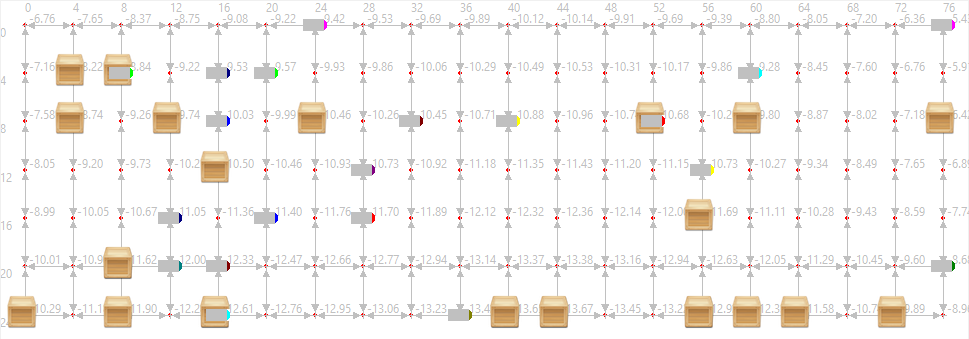
\includegraphics[width=0.9\textwidth]{thewarehouse.png}
    \caption{The warehouse in which the experiments are set}
    \label{fig:thewarehouse}
\end{figure}

\subsection{Miscellaneous variables}
There are some variables that may have an impact on experiment results but which are not directly related to the domain of discourse, i.e. configuration of the gradient field. There are the following:

\begin{itemize}
    \item Number of agents: there are always 20 agents
    \item Size of the warehouse: 8 rows by 20 columns, with roles assigned to the different rows as specified in section \ref{sec:setup}
    \item Time-out threshold: Some states of the traffic jam protocol maintain a time-out counter, performing an action when there is a time-out (refer to section \ref{sec:agentarch} for more details). Currently, this threshold is set to 0 milliseconds, which means that agents send out messages virtually every tick.
    \item Base strength of the agents' repulsive field: set to 0.25.
    \item Base strength of the parcels' attractive field: set to 1.
\end{itemize}

\subsection{Performed experiments}